\documentclass{standalone}
\usepackage{tikz}
\usetikzlibrary{patterns, positioning}

\begin{document}
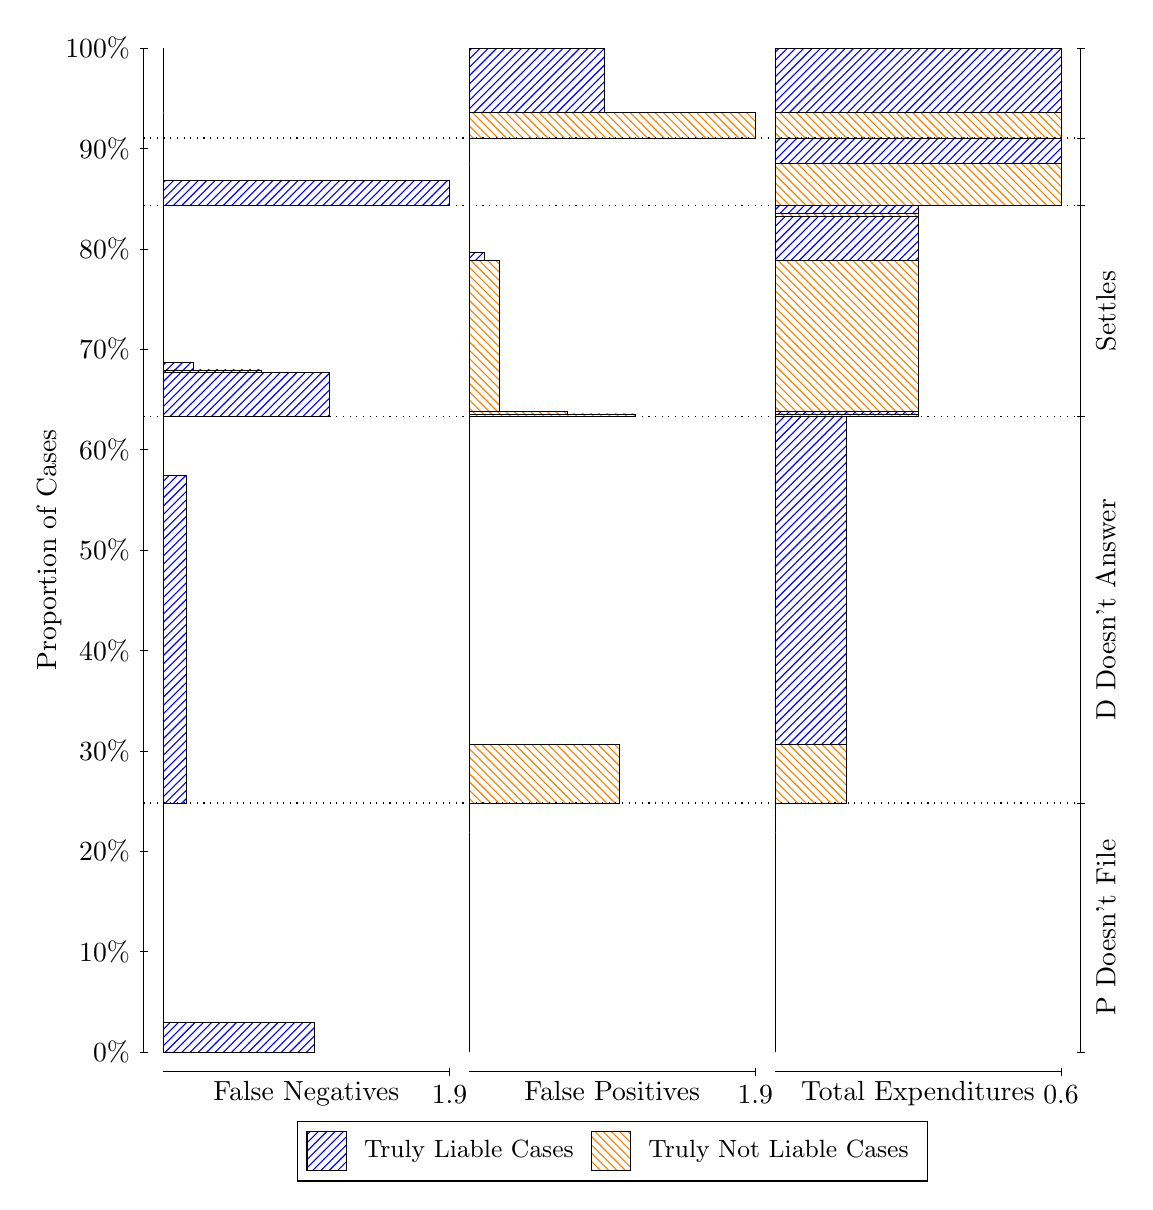
\begin{tikzpicture}
\draw[black, very thin] (1.5,1.75) -- (1.5,14.5);
\node[rotate=90, anchor=center] at (0.3, 8.125) {Proportion of Cases};
\draw[black, very thin] (1.45,1.75) -- (1.55,1.75);
\node[anchor=east] at (1.45, 1.75) {0\%};
\draw[black, very thin] (1.45,3.025) -- (1.55,3.025);
\node[anchor=east] at (1.45, 3.025) {10\%};
\draw[black, very thin] (1.45,4.3) -- (1.55,4.3);
\node[anchor=east] at (1.45, 4.3) {20\%};
\draw[black, very thin] (1.45,5.575) -- (1.55,5.575);
\node[anchor=east] at (1.45, 5.575) {30\%};
\draw[black, very thin] (1.45,6.85) -- (1.55,6.85);
\node[anchor=east] at (1.45, 6.85) {40\%};
\draw[black, very thin] (1.45,8.125) -- (1.55,8.125);
\node[anchor=east] at (1.45, 8.125) {50\%};
\draw[black, very thin] (1.45,9.4) -- (1.55,9.4);
\node[anchor=east] at (1.45, 9.4) {60\%};
\draw[black, very thin] (1.45,10.675) -- (1.55,10.675);
\node[anchor=east] at (1.45, 10.675) {70\%};
\draw[black, very thin] (1.45,11.95) -- (1.55,11.95);
\node[anchor=east] at (1.45, 11.95) {80\%};
\draw[black, very thin] (1.45,13.225) -- (1.55,13.225);
\node[anchor=east] at (1.45, 13.225) {90\%};
\draw[black, very thin] (1.45,14.5) -- (1.55,14.5);
\node[anchor=east] at (1.45, 14.5) {100\%};

\draw[black, very thin] (13.4,1.75) -- (13.4,14.5);
\draw[black, very thin] (13.35,1.75) -- (13.45,1.75);
\node[anchor=west] at (13.35, 1.75) {};
\draw[black, very thin] (13.35,4.9119) -- (13.45,4.9119);
\node[anchor=west] at (13.35, 4.9119) {};
\draw[black, very thin] (13.35,9.8176) -- (13.45,9.8176);
\node[anchor=west] at (13.35, 9.8176) {};
\draw[black, very thin] (13.35,12.5) -- (13.45,12.5);
\node[anchor=west] at (13.35, 12.5) {};
\draw[black, very thin] (13.35,13.358) -- (13.45,13.358);
\node[anchor=west] at (13.35, 13.358) {};
\draw[black, very thin] (13.35,14.5) -- (13.45,14.5);
\node[anchor=west] at (13.35, 14.5) {};

\draw[black, very thin, pattern color=blue, pattern=north east lines] (1.75,1.75) rectangle (3.6623,2.1272);
\draw[black, very thin, pattern color=orange, pattern=north west lines] (1.75,2.1272) rectangle (1.75,4.9119);
\draw[black, very thin, pattern color=blue, pattern=north east lines] (1.75,4.9119) rectangle (2.0368,9.0737);
\draw[black, very thin, pattern color=orange, pattern=north west lines] (1.75,9.0737) rectangle (1.75,9.8176);
\draw[black, very thin, pattern color=blue, pattern=north east lines] (1.75,9.8176) rectangle (3.8535,10.384);
\draw[black, very thin, pattern color=blue, pattern=north east lines] (1.75,10.384) rectangle (2.993,10.412);
\draw[black, very thin, pattern color=blue, pattern=north east lines] (1.75,10.412) rectangle (2.1325,10.511);
\draw[black, very thin, pattern color=orange, pattern=north west lines] (1.75,10.511) rectangle (1.75,12.5);
\draw[black, very thin, pattern color=blue, pattern=north east lines] (1.75,12.5) rectangle (5.3833,12.821);
\draw[black, very thin, pattern color=orange, pattern=north west lines] (1.75,12.821) rectangle (1.75,13.358);
\draw[black, very thin, pattern color=orange, pattern=north west lines] (1.75,13.358) rectangle (1.75,13.679);
\draw[black, very thin, pattern color=blue, pattern=north east lines] (1.75,13.679) rectangle (1.75,14.5);
\draw[black, very thin, pattern color=orange, pattern=north west lines] (5.6333,1.75) rectangle (5.6333,4.5347);
\draw[black, very thin, pattern color=blue, pattern=north east lines] (5.6333,4.5347) rectangle (5.6333,4.9119);
\draw[black, very thin, pattern color=orange, pattern=north west lines] (5.6333,4.9119) rectangle (7.5456,5.6557);
\draw[black, very thin, pattern color=blue, pattern=north east lines] (5.6333,5.6557) rectangle (5.6333,9.8176);
\draw[black, very thin, pattern color=orange, pattern=north west lines] (5.6333,9.8176) rectangle (7.7368,9.8534);
\draw[black, very thin, pattern color=orange, pattern=north west lines] (5.6333,9.8534) rectangle (6.8763,9.8895);
\draw[black, very thin, pattern color=orange, pattern=north west lines] (5.6333,9.8895) rectangle (6.0158,11.807);
\draw[black, very thin, pattern color=blue, pattern=north east lines] (5.6333,11.807) rectangle (5.8246,11.906);
\draw[black, very thin, pattern color=blue, pattern=north east lines] (5.6333,11.906) rectangle (5.6333,12.5);
\draw[black, very thin, pattern color=orange, pattern=north west lines] (5.6333,12.5) rectangle (5.6333,13.036);
\draw[black, very thin, pattern color=blue, pattern=north east lines] (5.6333,13.036) rectangle (5.6333,13.358);
\draw[black, very thin, pattern color=orange, pattern=north west lines] (5.6333,13.358) rectangle (9.2667,13.679);
\draw[black, very thin, pattern color=blue, pattern=north east lines] (5.6333,13.679) rectangle (7.3544,14.5);
\draw[black, very thin, pattern color=orange, pattern=north west lines] (9.5167,1.75) rectangle (9.5167,4.5347);
\draw[black, very thin, pattern color=blue, pattern=north east lines] (9.5167,4.5347) rectangle (9.5167,4.9119);
\draw[black, very thin, pattern color=orange, pattern=north west lines] (9.5167,4.9119) rectangle (10.425,5.6557);
\draw[black, very thin, pattern color=blue, pattern=north east lines] (9.5167,5.6557) rectangle (10.425,9.8176);
\draw[black, very thin, pattern color=orange, pattern=north west lines] (9.5167,9.8176) rectangle (11.333,9.8536);
\draw[black, very thin, pattern color=blue, pattern=north east lines] (9.5167,9.8536) rectangle (11.333,9.8814);
\draw[black, very thin, pattern color=orange, pattern=north west lines] (9.5167,9.8814) rectangle (11.333,11.799);
\draw[black, very thin, pattern color=blue, pattern=north east lines] (9.5167,11.799) rectangle (11.333,12.365);
\draw[black, very thin, pattern color=orange, pattern=north west lines] (9.5167,12.365) rectangle (11.333,12.401);
\draw[black, very thin, pattern color=blue, pattern=north east lines] (9.5167,12.401) rectangle (11.333,12.5);
\draw[black, very thin, pattern color=orange, pattern=north west lines] (9.5167,12.5) rectangle (13.15,13.036);
\draw[black, very thin, pattern color=blue, pattern=north east lines] (9.5167,13.036) rectangle (13.15,13.358);
\draw[black, very thin, pattern color=orange, pattern=north west lines] (9.5167,13.358) rectangle (13.15,13.679);
\draw[black, very thin, pattern color=blue, pattern=north east lines] (9.5167,13.679) rectangle (13.15,14.5);
\draw[black, dotted] (1.5,4.9119) -- (13.4,4.9119);
\draw[black, dotted] (1.5,9.8176) -- (13.4,9.8176);
\draw[black, dotted] (1.5,12.5) -- (13.4,12.5);
\draw[black, dotted] (1.5,13.358) -- (13.4,13.358);
\draw[black, very thin] (1.75,1.5) -- (5.3833,1.5);
\node[anchor=north] at (3.5667, 1.5) {False Negatives};
\draw[black, very thin] (5.3833,1.45) -- (5.3833,1.55);
\node[anchor=north] at (5.3833, 1.45) {1.9};

\draw[black, very thin] (5.6333,1.5) -- (9.2667,1.5);
\node[anchor=north] at (7.45, 1.5) {False Positives};
\draw[black, very thin] (9.2667,1.45) -- (9.2667,1.55);
\node[anchor=north] at (9.2667, 1.45) {1.9};

\draw[black, very thin] (9.5167,1.5) -- (13.15,1.5);
\node[anchor=north] at (11.333, 1.5) {Total Expenditures};
\draw[black, very thin] (13.15,1.45) -- (13.15,1.55);
\node[anchor=north] at (13.15, 1.45) {0.6};

\node[black, centered, rotate=90] at (13.72, 3.3309) {P Doesn't File};
\node[black, centered, rotate=90] at (13.72, 7.3647) {D Doesn't Answer};
\node[black, centered, rotate=90] at (13.72, 11.159) {Settles};



\draw (7.449999999999999,1.5) node[draw=none] (baseCoordinate) {};
\begin{scope}[align=center]
        \matrix[scale=0.5, draw=black, below=0.5cm of baseCoordinate, nodes={draw}, column sep=0.1cm]{
            \node[rectangle, draw, minimum width=0.5cm, minimum height=0.5cm, pattern=north east lines, pattern color=blue] {}; &
            \node[draw=none, font=\small] (B) {Truly Liable Cases}; &
            \node[rectangle, draw, minimum width=0.5cm, minimum height=0.5cm, pattern=north west lines, pattern color=orange] {}; &
            \node[draw=none, font=\small] (B) {Truly Not Liable Cases}; \\
            };
\end{scope}

\end{tikzpicture}
\end{document}